\documentclass[8pt,landscape]{article}

% PACKAGES
\usepackage[letterpaper, margin=0.1in]{geometry}
\usepackage{amsmath, amssymb, geometry}
\usepackage{multicol}
\usepackage{setspace}
\usepackage{sectsty}
\usepackage{verbatim}
\usepackage{graphicx}
\usepackage{xcolor}
\usepackage{listings}
\usepackage{enumitem}
\usepackage{booktabs} % For better tables if needed

% Define a custom color for code highlighting and environment
\definecolor{myred}{RGB}{204, 0, 0} % A strong red
\definecolor{mygray}{RGB}{240, 240, 240} % Light gray for background
\setlist[itemize]{
    noitemsep,  % Removes vertical space between list items
    topsep=0pt,  % Removes space before the list
    partopsep=0pt, % Removes extra space when a list begins mid-paragraph
    parsep=0pt, % Removes space between paragraphs within an item
    leftmargin=*, % Sets the left margin to the minimum necessary
    labelsep=0.5em, % You can slightly adjust the space between the bullet and the text
}
% LISTINGS SETUP for R and Python
\lstset{
  basicstyle=\ttfamily\scriptsize\color{black},
  backgroundcolor=\color{mygray},
  frame=single,
  frameround=tttt,
  framesep=0pt,        % no padding between code and frame
  rulecolor=\color{black!20},
  rulesep=0pt,         % no space between rules
  breaklines=true,
  columns=fullflexible,
  showstringspaces=false,
  commentstyle=\color{gray},
  keywordstyle=\color{blue!80!black},
  stringstyle=\color{myred},
  breakatwhitespace=true,
  xleftmargin=0pt,     % no left margin
  xrightmargin=0pt,    % no right margin
  aboveskip=0pt,       % no space above listing
  belowskip=0pt,       % no space below listing
  abovecaptionskip=0pt,
  belowcaptionskip=0pt,
  framexleftmargin=0pt,
  framexrightmargin=0pt,
  framextopmargin=0pt,
  framexbottommargin=0pt
}

% FORMATTING
\setstretch{0.9} % Reduce line spacing
\setlength{\parindent}{0pt}
\setlength{\parskip}{0pt}

% Reduce section spacing and change color
\makeatletter
\renewcommand{\section}{\@startsection{section}{2}{0pt}%
    {0.1ex}% space before section
    {0.1ex}% space after section
    {\fontsize{8}{9}\bfseries\color{red}}} % section font: 8pt
\makeatother

% Reduce subsection spacing and make subsections blue
\makeatletter
\renewcommand{\subsection}{\@startsection{subsection}{2}{0pt}%
    {0.1ex}% space before subsection
    {0.1ex}% space after subsection
    {\fontsize{8}{9}\bfseries\color{blue}}} % Subsection font: 8pt
\makeatother

% Custom command for red-highlighted code/commands (for in-line use)
\newcommand{\code}[1]{\textcolor{myred}{\texttt{#1}}}

% Custom small text wrapper - ensuring 8pt for body text
\newcommand{\smalltext}[1]{
  {\fontsize{8}{9}\selectfont\sloppy #1\par}
}

% DOCUMENT START
\begin{document}
\fontsize{8}{9}\selectfont % Set the base font size to 8pt and line skip to 9pt for the entire document
\pagestyle{empty}
\begin{multicols}{3}


\section{Common applications of clustering}
\smalltext{
  Clustering is the task of partitioning the dataset into groups called clusters based on their similarities.
   Data exploration, clustering/grouping of data points, Customer segmentation, Social network analysis, Medical imaging, Imputing missing data, data compression, privacy preservation
  }
\section{K-Means clustering }
\smalltext{
  Clustering is based on the notion of similarity or distances between points.
  K - number of clusters.
}
\begin{lstlisting}[language=python]
  from sklearn.cluster import KMeans
  kmeans = KMeans(n_clusters=3, n_init='auto')
  kmeans.fit(X); # Passing X because this is unsupervised learning
  clust_labels = kmeans.predict(X)
  kmeans.labels_ #attribute of KMeans object.
\end{lstlisting}

\subsection{Algorithm}
\smalltext{
\textbf{Input:} Data points X and the number of clusters K

\textbf{Initialization:} K initial centers for the clusters

\textbf{Iterative process:} repeat - Assign each example to the closest center. - Estimate new centers as average of observations in a cluster.
until centers stop changing or maximum iterations have reached.
}

\subsection{Initialization}
\smalltext{
  The initialization is stochastic - random.
  Makes sense to have K $\le$ no. of examples.
  Sensitive to initialization and the solution may change depending upon the initialization.
  Terminates when the centroid locations do not change between iterations.
}

\subsection{choosing k}
\smalltext{
  In supervised setting we carried out hyperparameter optimization based on cross-validation scores.
Since in unsupervised learning we do not have the target values, it becomes difficult to objectively measure the effectiveness of the algorithms.
There is no definitive or satisfactory approach.

\textbf{Method 1: The Elbow method} | method looks at the sum of intra-cluster distances, which is also referred to as inertia. The inertia decreases as K increases. If I have number of clusters = number of examples, each example will have its own cluster and the intra-cluster distance will be 0.
Instead we evaluate the trade-off: “small k” vs “small intra-cluster distances”.


\textbf{Method 2: The Silhouette method} | Not dependent on the notion of cluster centers.
Distance for a data point the difference between the  \textbf{mean intra-cluster distance (a)} and the \textbf{mean nearest-cluster distance (b)} for each sample.
$s = \frac{b - a}{\max(a, b)}$ Best value = 1 | worst value = -1 (between 1 and -1)

\textbf{Imp:} Thickness of each silhouette represents the size of that cluster. The length (or area) of each silhouette indicates the “goodness” of each cluster.
A slower dropoff (more rectangular) indicates more points are “happy” in their cluster. 
The red dashed line shows the average silhouette score for all samples, which tells you the overall clustering fit. The close this score is to 1, the better the clustering fit is.
For a well-fitted clustering model, expect to see the silhouette plots for each cluster above the average silhouette score line, and with widths which do not vary wildly.

\textbf{Limitations:} The subjectivity in identifying the “elbow” point, which is not always clear-cut.
A focus on variance reduction without directly measuring the quality of the clustering.
Challenges in interpreting the overall clustering quality in cases where clusters have a mix of positive and negative silhouette values.
The potential inability of silhouette plots to effectively capture the performance of the clustering algorithm in datasets with complex shapes or varying densities.
}


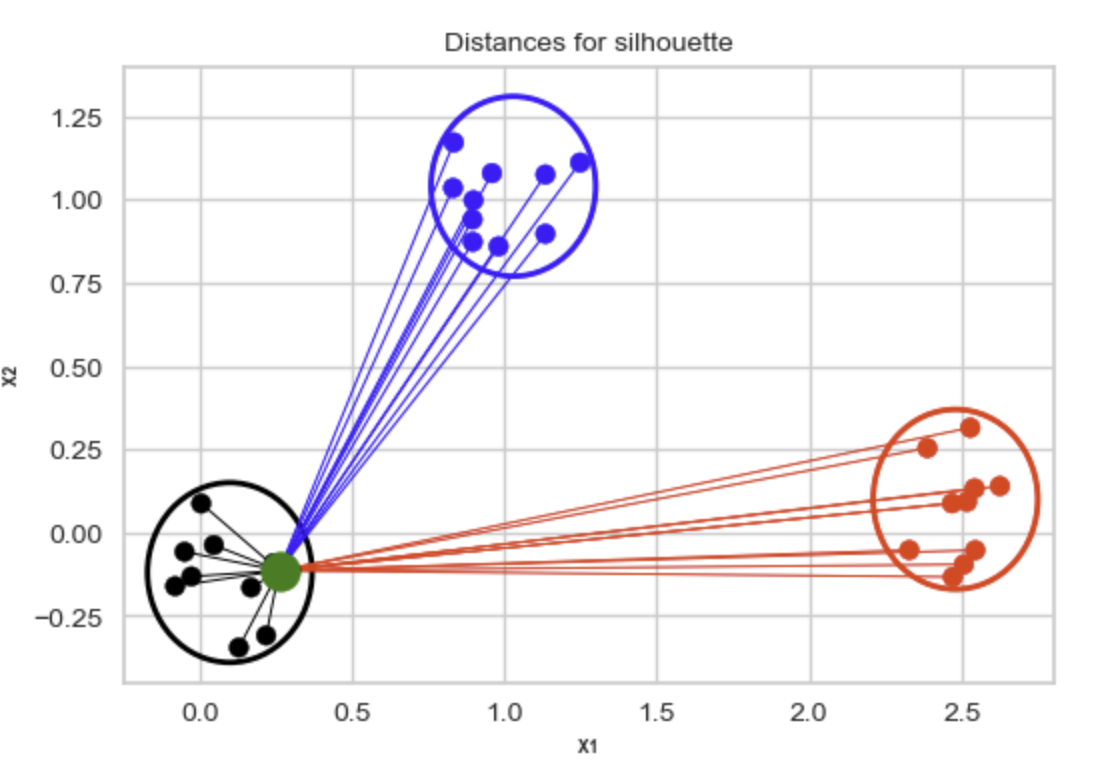
\includegraphics[width=0.5\linewidth, height=2cm]{silllo.png}
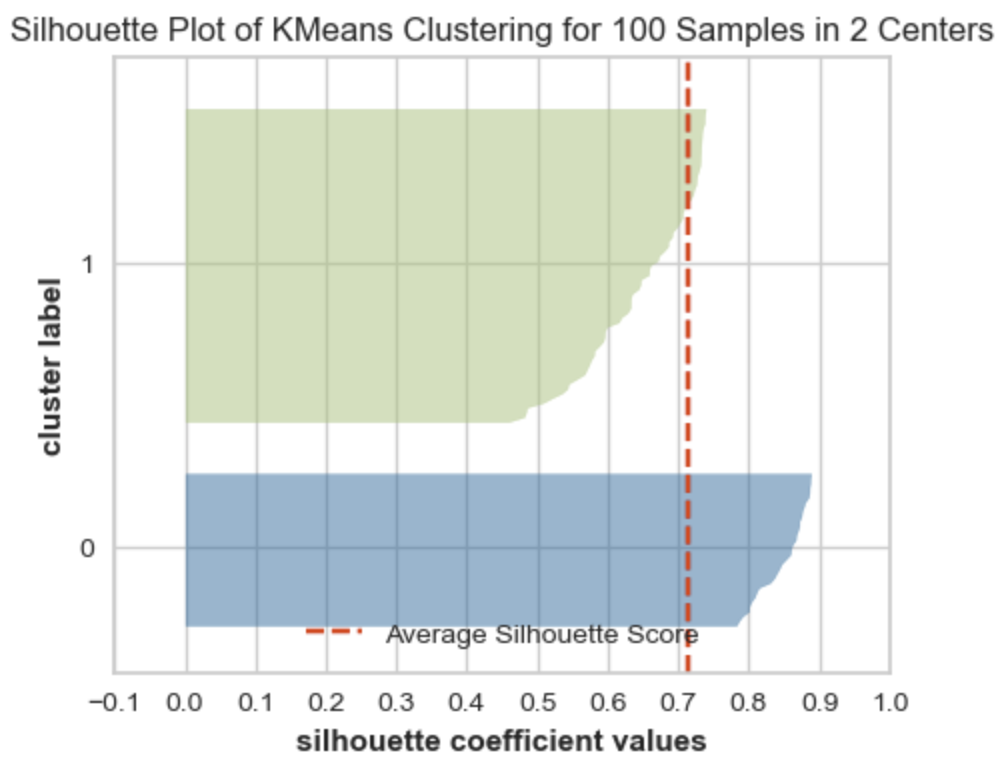
\includegraphics[width=0.5\linewidth, height=2cm]{silllo-2.png}


\end{multicols}
\end{document}
